\documentclass[12pt]{article}
\usepackage[a4paper, total={6in, 9in}]{geometry}
\usepackage{graphicx}
\graphicspath{ {./images/output/} }
\usepackage{caption}
\usepackage[english]{babel}
\usepackage{titling}
\usepackage{float}
% \usepackage{amsmath}
\usepackage{minted}
\usepackage{multicol}
% \usepackage{array}
% \usepackage{setspace}
% \usepackage{placeins}
\setlength{\parindent}{0pt}

% \usepackage{lipsum}

\title{Analog Signal Transmission and Reception}
\author{}
\date{}

\pagenumbering{gobble}
\begin{document}
\vspace*{\fill}
\begin{center}

    \emph{Heaven's Light is Our Guide} \\
    \textbf{Rajshahi University of Engineering and Technology} \\

    \begin{figure}[H]
        \centering
        
\includegraphics[scale=.34]{images/RUET_logo.png}
        \label{fig:ruet_logo}
    \end{figure}
    \vspace{5mm}

    \textbf{Course Code}\\
    ECE 3208\\
    \vspace{3mm}
    \textbf{Course Title}\\
    Communication Engineering Sessional

    \vspace{5mm}
    \textbf{Experiment Date:} {January 21, 2025},\\
    \textbf{Submission Date:} {February 11, 2025}\\

    \vspace{5mm}
    \textbf{Lab Report 3: \\
        Determination of Modulation Index of FM Wave}

    \vspace{15mm}

    \begin{tabular}{c|c}
        \textbf{Submitted to} & \textbf{Submitted by} \\
        Dr. Md. Kamal Hosain  & Md. Tajim An Noor     \\
        Professor             & Roll: 2010025         \\
        Dept of ETE, RUET     &                       \\
    \end{tabular}

\end{center}
\vspace*{\fill}


\pagebreak

\tableofcontents

\pagebreak
\pagenumbering{arabic}
\maketitle

\section*{Theory}
\addcontentsline{toc}{section}{Theory}
Analog signal transmission and reception are fundamental concepts in communication engineering. Analog signals are continuous signals that vary over time and can take any value within a given range. These signals are used to transmit information such as audio, video, and other data over various mediums like air, cables, and optical fibers \cite{haykin2001communication}. In this experiment, we focus on Amplitude Modulation (AM) and demodulation.
\\\\
\textbf{Amplitude Modulation (AM)}: In AM, the amplitude of the carrier wave is varied in proportion to the information signal. This technique is widely used in radio broadcasting \cite{sklar2001digital}.
\\\\
The reception of analog signals involves demodulation, which is the process of extracting the original information signal from the modulated carrier wave. This is achieved using various demodulation techniques corresponding to the modulation methods used during transmission \cite{sklar2001digital}.

\begin{figure}[H]
    \centering
    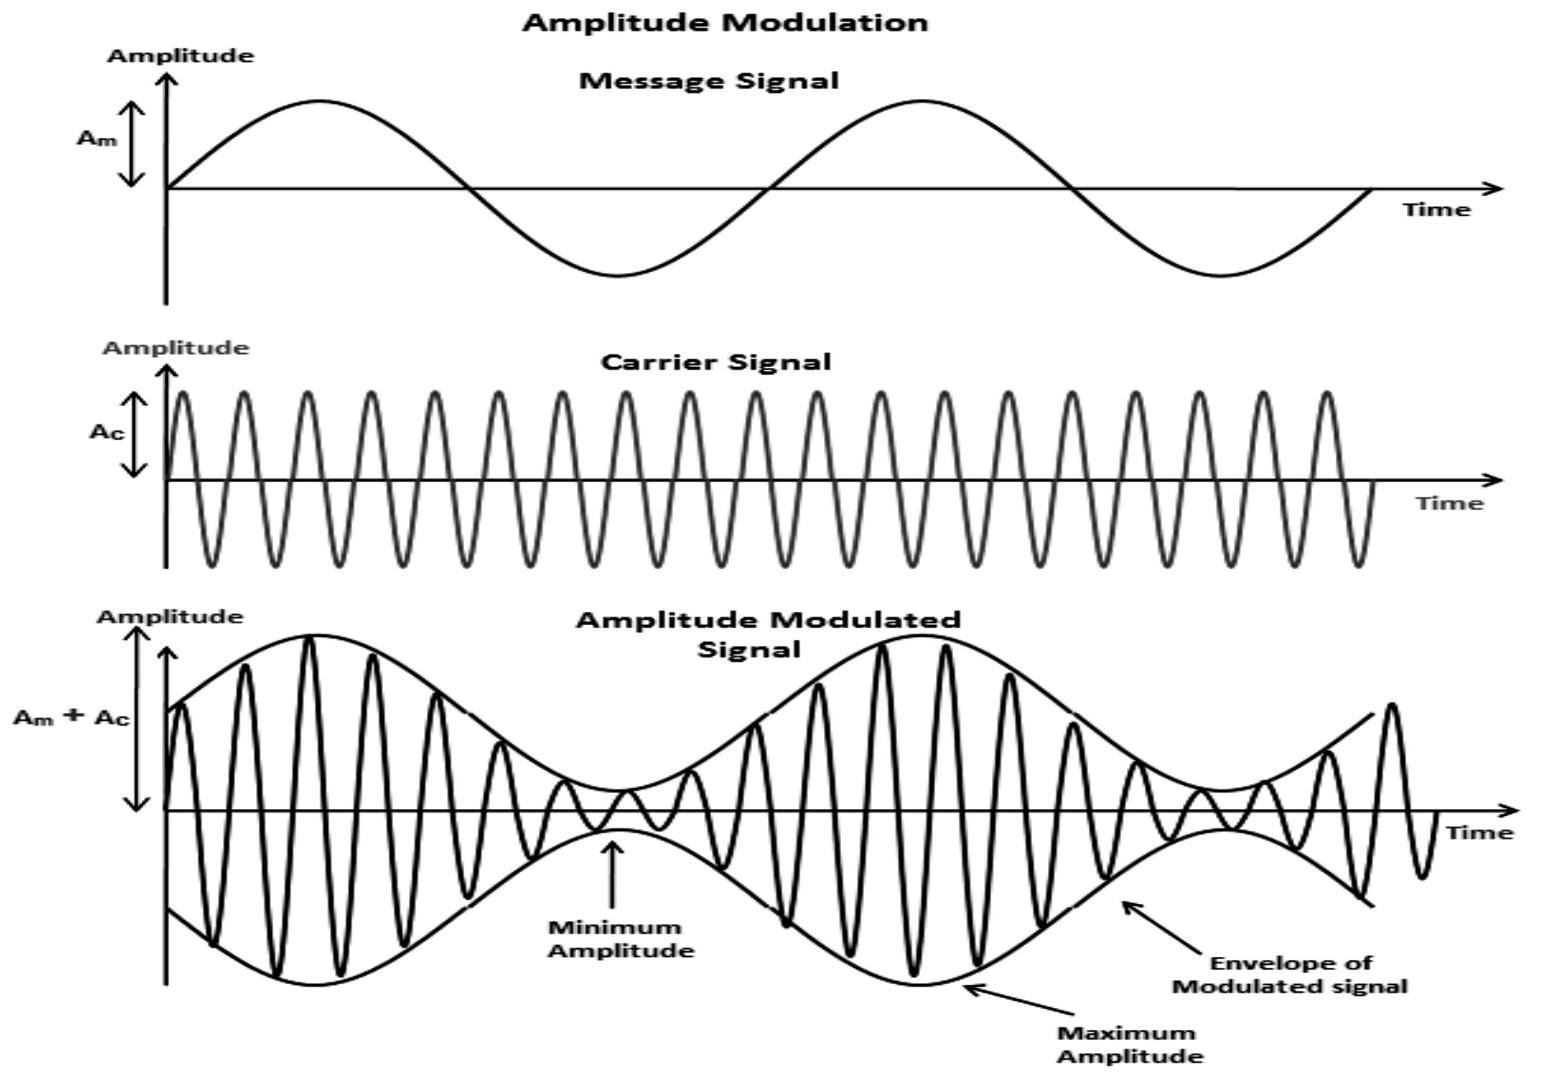
\includegraphics[width=0.6\textwidth]{amMod.png}
    \caption{Illustration of Signals and Amplitude Modulation (AM)\cite{pic}}
    \label{fig:signals_am_mod}
\end{figure}

Analog signal transmission and reception are susceptible to noise and interference, which can degrade the quality of the received signal. Techniques such as filtering and amplification are employed to mitigate these effects and improve signal quality \cite{haykin2001communication}.
\\\\
Overall, understanding analog signal transmission and reception is crucial for designing and analyzing communication systems that rely on analog signals \cite{proakis2007digital}.

\section*{Required Apparatus}
\addcontentsline{toc}{section}{Required Apparatus}
\begin{itemize}
    \item  Analogue Signal Processing (Model No. DL 3155M60R)
    \item Oscilloscope
    \item Connecting Wires
\end{itemize}

\section*{Block Diagram}
\addcontentsline{toc}{section}{Block Diagram}
\begin{figure}[H]
    \centering
    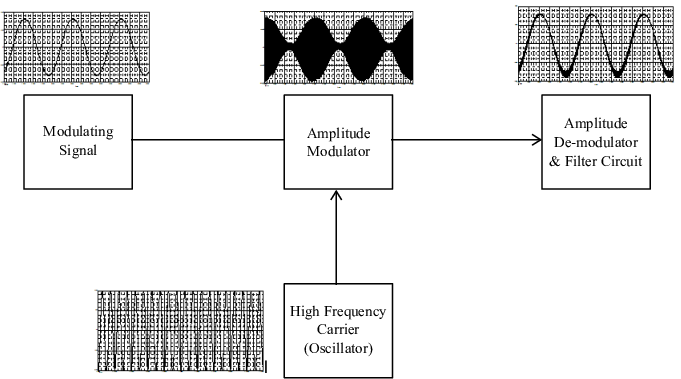
\includegraphics[width=0.8\textwidth]{blck.png}
    \caption{Block diagram of Amplitude Modulation and Demodulation.\cite{blck}}
    \label{fig:block_diagram}
\end{figure}

\section*{Procedure}
\addcontentsline{toc}{section}{Procedure}
\begin{enumerate}
    \item The Analogue Signal Processing board (Model No. DL 3155M60R) was connected to the power supply.
    \item An analog signal was generated using the signal generator on the Analogue Signal Processing board.
    \item The output of the signal generator was connected to the input of the modulator section on the board.
    \item The modulator was set to perform Amplitude Modulation (AM) using the carrier signal provided by the board.
    \item The waveform of the message signal and the modulated signal was observed and recorded using the oscilloscope.
    \item The output of the modulator was connected to the input of the demodulator section on the board.
    \item The modulated signal was demodulated to retrieve the original message signal.
    \item The demodulated signal was passed through a filter to remove any noise and interference.
    \item The waveform of the demodulated signal was observed and recorded using the oscilloscope.
    \item The waveforms of the original message signal, the modulated signal, and the demodulated signal were compared.
\end{enumerate}

\section*{Matlab Simulation}
\addcontentsline{toc}{section}{Matlab Simulation}

\subsection*{Code:}
\addcontentsline{toc}{subsection}{Code}
The following Matlab code simulates the generation, modulation, and demodulation of an analog signal using Amplitude Modulation (AM).

\inputminted[linenos,breaklines,breakanywhere]{matlab}{./assets/analogMod.m}

\section*{Output}
\addcontentsline{toc}{section}{Output}

\subsection*{Experiment Outputs}
\addcontentsline{toc}{subsection}{Experiment Outputs}
\begin{figure}[H]
    \centering
    \begin{minipage}{0.45\textwidth}
        \centering
        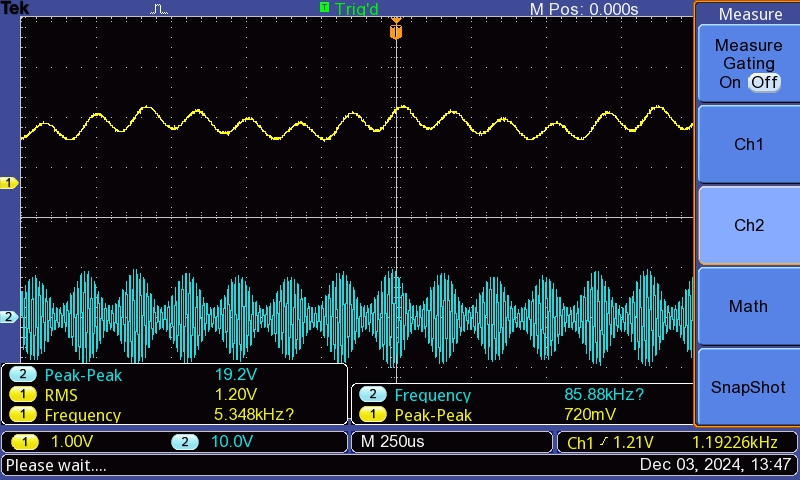
\includegraphics[width=\textwidth]{Lr1-1-msg-mod.JPG}
        \caption{Waveform of the Original Message Signal (Yellow) and the Modulated Signal (Blue)}
        \label{fig:original_message_signal}
    \end{minipage}
    \hfill
    \begin{minipage}{0.45\textwidth}
        \centering
        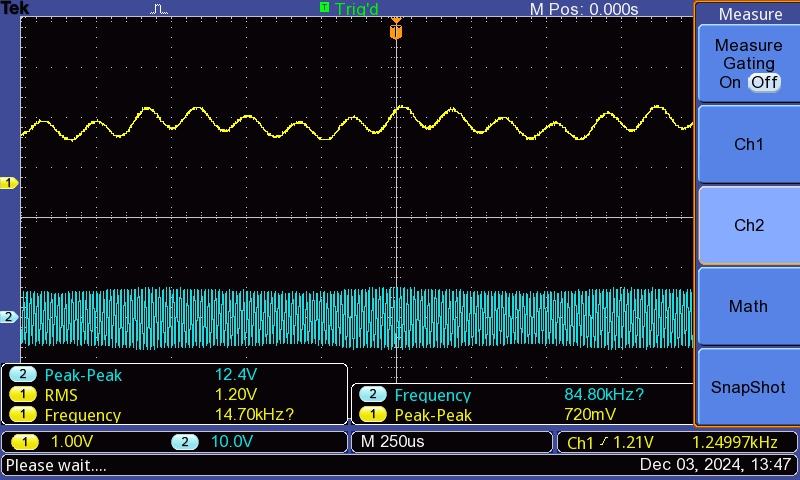
\includegraphics[width=\textwidth]{Lr1-4-msg-mod2.JPG}
        \caption{Waveform of the Modulated Signal (Yellow) and the Modulated Signal (Blue) with different message signal}
        \label{fig:modulated_signal}
    \end{minipage}
\end{figure}

\begin{figure}[H]
    \centering
    \begin{minipage}{0.45\textwidth}
        \centering
        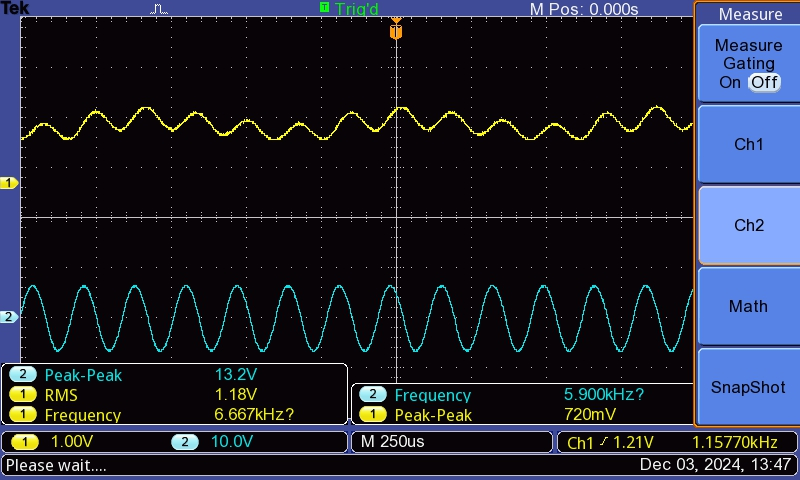
\includegraphics[width=\textwidth]{Lr1-3-msg-tr-msg.JPG}
        \caption{Waveform of the original message signal (Yellow) and the demodulated signal (Blue)}
        \label{fig:demodulated_signal}
    \end{minipage}
\end{figure}

\subsection*{Matlab Simulation Outputs}
\addcontentsline{toc}{subsection}{Matlab Simulation Outputs}
\begin{figure}[H]
    \centering
    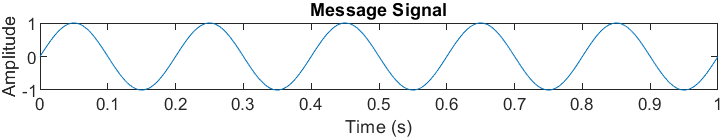
\includegraphics[width=\textwidth]{msg.png}
    \caption{Original Message Signal}
    \label{fig:simulation_message_signal}
\end{figure}

\begin{figure}[H]
    \centering
    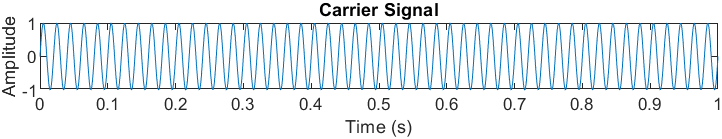
\includegraphics[width=\textwidth]{car.png}
    \caption{Carrier Signal}
    \label{fig:simulation_carrier_signal}
\end{figure}

\begin{figure}[H]
    \centering
    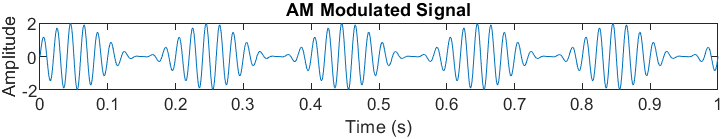
\includegraphics[width=\textwidth]{mod.png}
    \caption{Modulated Signal}
    \label{fig:simulation_modulated_signal}
\end{figure}

\begin{figure}[H]
    \centering
    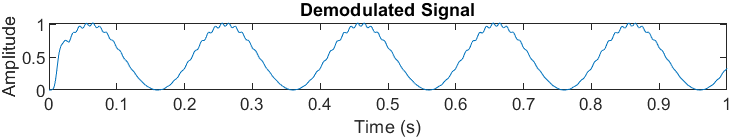
\includegraphics[width=\textwidth]{demod.png}
    \caption{Demodulated Signal}
    \label{fig:simulation_demodulated_signal}
\end{figure}

\section*{Discussion}
\addcontentsline{toc}{section}{Discussion}
The experiment and Matlab simulation demonstrate the process of analog signal transmission and reception using Amplitude Modulation (AM). The original message signal is modulated by varying the amplitude of the carrier signal, resulting in the modulated signal. The modulated signal is then demodulated to retrieve the original message signal.
\\\\
The waveforms of the original message signal, the modulated signal, and the demodulated signal are observed and compared. The demodulated signal closely resembles the original message signal, demonstrating the effectiveness of the demodulation process.

\section*{Precautions \& Conclusion}
\addcontentsline{toc}{section}{Precautions \& Conclusion}
\subsection*{Precautions:}
\begin{itemize}
    \item All connections were ensured to be secure before powering on the equipment to avoid short circuits or damage.
    \item The signal generator settings were verified to ensure the correct frequency and amplitude were used for modulation.
    \item The oscilloscope probes were handled carefully to avoid damaging the equipment or the circuit.
    \item Live wires or terminals were avoided to prevent electric shock.
    \item The modulator and demodulator settings were double-checked to ensure accurate modulation and demodulation.
    \item The work area was kept clean and organized to prevent accidental disconnections or interference.
    \item The manufacturer's guidelines for operating the Analogue Signal Processing board and other equipment were followed.
\end{itemize}

\subsection*{Conclusion:}
Analog signal transmission and reception are essential concepts in communication engineering. The experiment and Matlab simulation provide a hands-on demonstration of Amplitude Modulation (AM) and the demodulation process. By observing the waveforms of the original message signal, the modulated signal, and the demodulated signal, we can understand the impact of modulation and demodulation on analog signals \cite{haykin2001communication}.
\\\\
The experiment highlights the importance of modulation techniques in transmitting information over various communication channels \cite{proakis2007digital}. It also emphasizes the need for demodulation to recover the original message signal from the modulated carrier wave. Overall, analog signal transmission and reception play a vital role in modern communication systems and are fundamental to the field of communication engineering \cite{sklar2001digital}.


\bibliographystyle{IEEEtran}
\renewcommand{\bibname}{References}
\addcontentsline{toc}{section}{References}
\bibliography{ref}

\end{document}
